\section{Déroulement du travail}

\subsection{Méthodologie et Organisation}

Durant toute la durée du stage, il y avait un suivi régulier, permettant une gestion de projet selon la méthode agile.

Chaque jour, une réunion d'alignement de 30 min s'appelant "Jour Fixe" avec mon équipe (dont mon tuteur), le SFDH, avait lieu.
Cela permettait à chaque membre de tenir les autres au courant de ce qu'il a fait la veille et de se faire aider par l'équipe en cas de questions.

Au début de chaque mois se déroulait additionnellement le Jour Fixe avec Stefan Bender, le responsable du département DSZ, afin d'aborder des points organisationnels et le tenir au courant du travail général de l'équipe du SFDH.

Un Jour Fixe DSZ se tenait tous les 3èmes mercredis du mois, avec l'ensemble du département, pour un alignement général des différents sous-départements. 

Au milieu du stage, un "Feedback Call" avec mon tuteur était l'occasion de partager mon ressenti sur le stage, ce que je voulais faire pendant les mois restants, si les projets précédents m'avaient plu, etc... 
Cela permettait aussi à mon tuteur de me donner son avis sur mon travail, et d'éventuellement m'indiquer les points à améliorer.
\\

Comme le travail avait lieu en hybride, toutes les réunions se faisaient en visio via Webex.
J'ai d'ailleurs bénéficié d'un ordinateur portable afin de pouvoir faire du télétravail plusieurs jours par semaine.
La communication avec les membres de la Bundesbank se faisait alors via la messagerie Jabber et par mail.
\\

Au niveau de l'organisation concernant purement mes tâches, le travail m'était toujours donné tâche par tâche, ce qui me permettait de ne pas être débordée et d'être aussi plus efficace.
De plus, cela encourage des réunions fréquentes et ainsi une gestion de projet agile.

Dès qu'une tâche était terminée, j'organisais une réunion d'avancement avec les personnes concernées pour avoir leur feedback ainsi que de nouvelles tâches.

\paragraph{Sécurité informatique}

S'agissant d'une grande banque centrale, la sécurité est bien sûr prioritaire. 
Les ordinateurs ne peuvent être connectés à internet seulement lorsqu'ils sont connectés au réseau de la Banque (directement ou par VPN), et seuls certains sites sont autorisés.

La Banque possède un serveur interne dans lequel tous les dossiers et fichiers sont partagés. 
Chaque dossier est protégé et n'est accessible qu'à certains groupes.

Si un nouveau logiciel a besoin d'être installé, il doit être commandé via la plateforme Servity, puis l'installation doit être déclenchée par le service IT.
De même pour certains accès, notamment pour Gitlab ou Python, qui sont à demander sur la plateforme BIAM.
\\

La mise en place de Python comprend notamment la création d'environnements virtuels pour chaque projet, afin d'éviter des problèmes aux changements de version de Python.

Heureusement, tout cela est très bien guidé sur Confluence, une plateforme de documentation partagée, où sont notamment disponibles des guides pour la mise en place de Python sur les machines de la banque.
Elle est également utilisée pour documenter certains projets avec l'état des lieux actuel, les recherches déjà effectuées, les étapes suivantes, etc...

% \pagebreak
\subsection{Application de la méthode et Résultats}

\subsubsection{Projet Gaia}

La toute première étape du projet était de participer à une réunion avec Manuel Fangmann, un membre du pôle Innovation de la Bundesbank, qui participait activement au projet durant l'ensemble de mon stage.
Le projet m'a donc été présenté et ma 1ère mission attribuée : Ecrire un code python qui parcourt les résultats Google avec comme entrée 'companyName + "sustainability reports" + year + "pdf"' et télécharger tous les pdf.

La liste d'entreprise est dans un premier temps celle du DAX40, qui réunit les 30 plus grandes entreprises cotées à la Bourse de Francfort.
J'ai décidé de tester la recherche avec une liste d'années allant de 2017 à 2022.

Il m'a été demandé de travailler sur mon ordinateur personnel pour ce projet, car étant donné que l'accès à la quasi-totalité des sites est bloqué sur les machine de la banque, il serait compliqué de téléchargé les pdfs depuis ces sites.
\\

En 2 jours, j'ai donc implémenté le Google Crawler à l'aide du package requests-html, et téléchargé les pdfs les plus pertinents, mais les résultats n'étaient pas des meilleurs. 
En effet, les résultats de recherche n'incluaient pas que des pdfs, et ceux trouvés n'étaient donc parfois pas les plus pertinents.
\\

J'ai ensuite tenté de récupérer les titres des PDFs ou des liens tels qu'ils sont indiqués pour les utilisateurs afin de pouvoir y lire le nom de l'entreprise et l'année, mais je n'ai pas réussi et cette entreprise était dans tous les cas inutile, puisque ces informations pouvaient souvent se trouver directement dans le lien.

Dans ma recherche d'amélioration, j'ai trouvé un package donnant des résultats plus pertinents : Beautiful Soup.
J'ai également mis en place un comptage des liens "douteux", c'est-à-dire ceux ne contenant ni le nom de la bonne entreprise, ni l'année.
Les différents liens sont désormais triés à la volée selon s'ils sont douteux ou non, et ces 2 listes ensuite sauvegardés dans le fichier json correspondant.
\\

Après la 1ère réunion d'avancement, j'ai mis en place beaucoup d'améliorations à mon code :
\begin{itemize}
    \item Calcul du pourcentage de pdfs justes trouvés par an
    \item Amélioration du tri des pdfs trouvés/non trouvés : Désormais, un pdf est défini comme douteux s'il ne contient pas l'année ET/OU pas le nom de l'entreprise, et non pas uniquement si aucun des deux n'est présent.
    \item Ajout d'un opérateur de recherche avancée pour n'obtenir que les les liens qui menant à un pdf (filetype:pdf) (-> il n'y a donc plus de rapports "not found", seulement des pdfs douteux)
    \item Parfois, seuls les 2 derniers chiffres de l'année sont notés dans le lien, ou encore l'une des deux parties du nom de la société (Ex: "Telekom" dans "Deutsche Telekom"), j'en ai donc tenu compte
    \item Un problème qui revenait assez fréquemment était que la bonne année pouvait être présente dans le lien, mais que dans le nom du fichier, une autre année était indiquée. Afin de passer en priorité l'année présente dans le nom du fichier, j'ai simplement vérifié que l'année était inscrite précisément à cet endroit, sans inspecter le reste du lien.
    \item les PDFs ne peuvent être définis comme trouvés uniquement si le lien contient le terme "Report"
\end{itemize}

La principale difficulté lors de la mise en place de ces améliorations était la gestion d'une condition très longue pour la définition d'un lien "non trouvé", qui est d'autant plus négative, avec à la fois des OR et AND.
J'ai finalement simplifié le résonnement en faisant un condition positive pour les liens "trouvés".
\\

Pour anticiper la suite du projet avec l'étape de Text Mining des PDFs, il m'a été demandé de tester l'extraction de textes et d'images des PDFs, ce que j'ai réussi sans difficulté avec le package Fitz.
\\

Concernant le téléchargement des PDFs, j'avais des difficultés à tous les télécharger, certains sites bloquant les requêtes lorsqu'elles sont détectées comme étant automatisées.
Cela se traduisait soit par une requête n'aboutissant jamais mais sans erreur, soit par un code de réponse "403-Forbidden".
Un autre cas d'impossibilité du téléchargement est lorsque les rapports sont incorporés à la page web, avec un "viewer intégré", ou encore lorsque le pdf n'est plus disponible sur la page en question.

J'ai pu résoudre le cas de requête infinie grâce à une liste de "User Agents" qui seraient choisis à chaque fois aléatoirement pour être inclus dans le header de la requête.
L'erreur 403 n'était en revanche pas solvable, même en tentant avec un Pool de Proxys. 
\\

Lors d'une réunion suivante, l'idée de lire les PDFs afin de mieux les classer a été suggérée. 
Je me suis donc attelée à cette tâche et ai extrait le texte des 3 premières pages des rapports dont le lien est douteux afin d'y chercher l'année, le nom de l'entreprise (ou partie du nom) et le terme "Sustainable Report" ou un dérivé.
Le lien était donc reclassé en conséquence.

Cela a considérablement amélioré les résultats, car ne considérer que le lien était très réducteur, et beaucoup de rapports douteux étaient en réalité justes.
Mais seules les 3 premières pages étaient optimales à lire, car après une autre année pouvait apparaître, bien qu'il s'agissait du rapport d'une autre année, faussant les résultats.
Lire moins de 3 pages était en revanche trop peu pour trouver toutes les informations requises.

Cette lecture de PDFs n'a cependant pas résolu tous les problèmes, bien qu'ils soient rares :
\begin{itemize}
    \item Le nom de l'entreprise ou même l'année ne sont parfois inscrits que sous forme d'image, non reconnue dans l'extraction de texte.
    \item L'année recherchée peut être écrite au début du rapport sans qu'il ne s'agisse du rapport de cette année-là. Celui-ci est donc noté comme trouvé alors qu'il est faux.
\end{itemize}

Après la prochaine réunion est venue l'étape de Refactoring du code, afin de 1-Rendre le code qui devenait de plus en plus fourni, plus lisible. 
2- Rendre les différentes étapes indépendantes les unes des autres.

Mon code pouvait être découpé en 5 parties : Préparation de la liste d'entrperises, Crawling (=recherche des liens), Téléchargement des pdfs, Lecture des fichiers, et écriture des statistiques finales des résultats trouvés.
Il y a donc 1 fichier par étape, en plus du Main qui les appelle toutes. 

Pour que toutes ces étapes soient plus indépendantes les unes des autres, il fallait que le tri des liens se fasse en deux temps : une première fois en même temps que le crawling, et une deuxième fois après la lecture automatique des rapports douteux.
J'ai donc 4 fichiers de résultats où se trouvent les différentes listes des liens obtenus pour chaque requête : found-list et doubt-list avant le téléchargement, et de même après le téléchargement.
Le fichier found-list après téléchargement est composé de la copie de la 1ère found-list, mais avec en plus de nouveaux liens qui étaient au départ douteux.
\\

La procédure est détaillée plus clairement ici :
\begin{figure}[H]
    \centering
    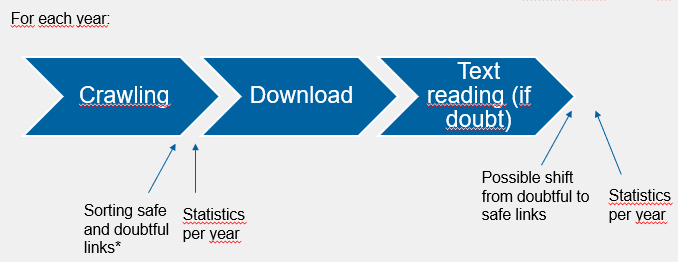
\includegraphics[width=\textwidth]{procedure.png}
    \caption{Procédure du code}
\end{figure}

Une fois que tout fonctionnait bien, il était temps de tester le code sur un volume beaucoup plus grand d'entreprises, à savoir la liste de celles du MSCI World, Index boursier pour les plus grandes entreprises dans le monde entier.
Cette liste en contient 3425 différentes. En ajoutant celles du DAX40, j'ai un échantillon de 3455 entreprises. 
Néanmoins, le fichier csv fourni contenait des doublons, et les noms des entreprises étaient parfois beaucoup trop longs (Ex : CONTEXTLOGIC INC CLASS A).
J'ai donc dans un premier temps fait une liste des termes "interdits" et ai tronqué les noms à partir de ces termes pour rendre une liste de noms propre (notamment "inc", "group", "plc", "class", etc.).

\begin{figure}[H]
    \centering
    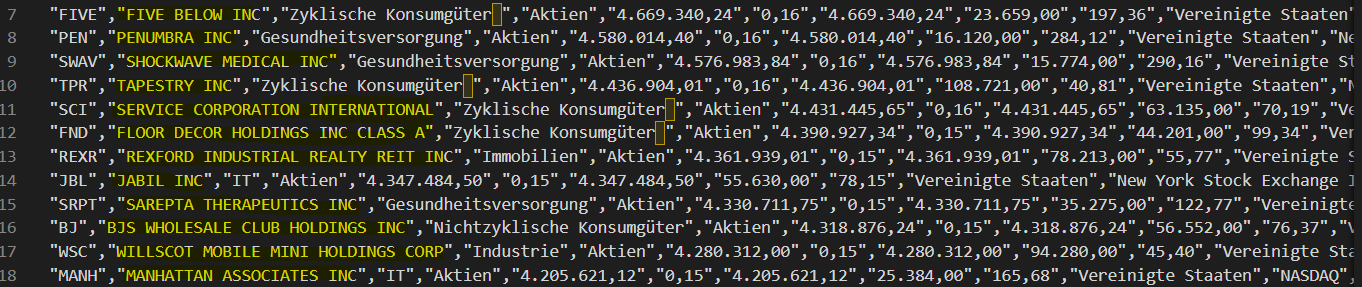
\includegraphics[width=\textwidth]{msci.png}
    \caption{Extrait de la liste MSCI avec les noms des entreprises en jaune}
\end{figure}

Pour ce projet, nous bénéficions d'une instance AWS Guacamole afin d'avoir une meilleure performance, le code étant très long à s'exécuter.
Mais tout ne s'est pas passé comme prévu : 
\begin{itemize}
    \item Lorsque mon code s'exécute sur l'instance, il s'arrête au bout de 5min avec une Exception provoquée par une réponse vide de Beautiful Soup.
    Je devais donc redémarrer l'instance afin que cela remarche, mais le problème revenait toujours, à une entreprise différente. En local, cela se produisait aussi, mais beaucoup plus tard.
    J'ai essayé de trouver une solution en cherchant un autre moyen de crawler, et suis tombée sur l'API Google Custom Search, qui fonctionnait beaucoup mieux avec des résultats fiables, mais qui avait un nombre de requêtes maximal par jour très bon pour la version gratuite.
    \item Le blocage du téléchargement que j'avais résolu en local, apparaissait sur l'instance de nouveau, ce qui bloquait l'ensemble du code.
\end{itemize}

J'ai donc organisé un court meeting afin de mettre l'équipe au courant de mes problèmes et de demander de l'aide.
Cette réunion m'a bien débloquée grâce aux solutions proposées :
En réalité, lorsque le code s'exécute rapidement, Beautiful Soup était "débordé" et n'avait pas toujours le temps de donner une réponse.
Avec un simple "time.sleep" de 0,8 secondes, le problème était résolu. La seule conséquence était que le temps d'exécution était un peu plus long.

Concernant le problème de téléchargement, j'ai mis en place un timeout et attrapé l'exception levée afin de continuer le code malgré tout. 
Les PDFs pour lesquels une exception a été levée sont sauvegardés dans un fichier afin de pouvoir les compter après-coup.
J'ai donc implémenté le calcul du pourcentage par an et du nombre total de PDFs n'ayant pas pu être téléchargés.
\\

Une journée de travail entière ne suffisant pas pour que le code s'exécute complètement, j'ai dû trouver une solution pour qu'il puisse reprendre là où il en etait lorsque l'instance se déconnecte ou que je dois fermer la page.

Parmi les différents changements à effectuer pour cela dans le programme, il fallait rendre les parties "web crawling" et "téléchargement/lecture des pdfs" complètement indépendantes l'une de l'autre.
Lors de la 1ère étape, au lieu de remplir des tableaux qui se vident à chaque nouvelle relance, il était pertinent de directement remplir les fichiers json (doubt-results0 ou found-results0) regroupant tous les liens trouvés ou non trouvés (ces fichiers n'étaient auparavent remplis qu'à la fin de chaque année parcourue). 
Ainsi à la 2ème étape, ces fichiers json pouvaient être lus pour trouver les liens et non dans les tables contenues dans les variables.
Ces liens étaient ensuite placés dans l'un des 2 nouveaux fichiers (doubt-results1 ou found-results1), au niveau de l'année courante.

\begin{figure}[H]
    \centering
    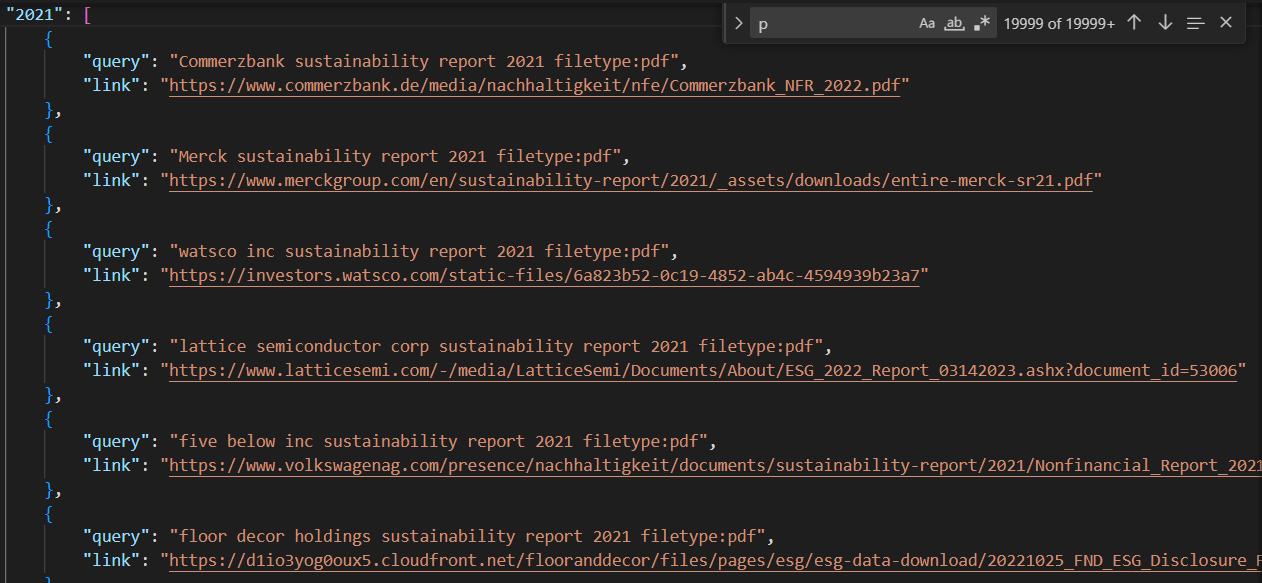
\includegraphics[width=\textwidth]{doubt_results_1.png}
    \caption{Extrait des résultats douteux après la lecture des pdfs (doubt-results-1.json)}
\end{figure}

La dernière entreprise traitée avec l'année en cours était notée dans un fichier txt lu à chaque nouvelle relance.
\\

En parcourant le fichier csv de la liste MSCI, j'ai remarqué que j'avais oublié beaucoup de termes interdits. 
Mais je devais à la fois vérifier que les rapports étaient toujours trouvés avec le nom de l'entreprise raccourci.
J'ai donc passé un petit temps à nettoyer les noms.
Un peu plus tard, j'ai remarqué que certaines entreprises avaient besoin des termes interdits pour être trouvées (Ex : Post holdings / software ag problem / fp corp).
J'ai donc modifié ma stratégie et ai instauré une liste de mots tolérés, et une de mots interdits. Ainsi, tous les termes après les mots tolérés sont supprimés (Ex : Tous ceux apres "inc").
Pour que la recherche du nom dans les rapports fonctionne toujours, j'ai mis en place la même règle que pour les liens : que seule une partie du nom peut être présente.
\\

J'ai donc pu tenter de lancer mon code pour de bon sur l'instance AWS, mais le fait d'y enregistrer les quelques 20 000 rapports dans le Repository Git posait problème, et plus aucune commande ne fonctionnait (git push, pull, add, status etc...).
Même en tentant de mettre en place git LFS, rien n'y faisait.
Afin de pouvoir accéder aux PDFs et étant donné que l'instance ne disposait que d'un terminal, j'ai pensé à uploader les PDFs directement sur Dropbox à la volée grâce à l'API, puisqu'ils devaient dans tous les cas y être à la fin.
Cela fonctionnait sur mon PC, mais pas sur l'instance, j'ai donc abandonné l'idée de l'utiliser. 
L'exécution était donc plus pratique et même plus réussie sur ma machine personnelle, le téléchargement étant moins souvent bloqué par les sites.

Alors que j'avais bien entamé l'exécution en local, j'ai remarqué que toutes les heures environ, le token expirait. Il fallait donc manuellement en regénérer un nouveau.
Il était donc finalement plus simple de d'enregistrer les PDFs en local et d'après coup tout uploader en même temps.
J'ai pu utiliser le forfait Business de Dropbox de mon tuteur pour y uploader les 136GB de PDFs.
\\

Les dernières observations que j'ai faites sur mes résultats, sont que :

1) Les résultats contenaient des doublons, soit à cause du fichier MSCI initial, soit quand je relançais le code, et qu'une entreprise qui avait déja été faite avant, soit refaite une 2ème fois.

2) qu'en fin de compte, le fait de considérer comme juste un lien qui contient les 2 derniers chiffres de l'année recherchée, faussait les résultats plus qu'autre chose :
certains liens contenaient juste une suite aléatoire de chiffres qui ne faisaient pas référence à l'année, et ils étaient considérés à tort comme justes.

J'ai donc supprimé cette condition, résolu le bug des doublons, et relancé le code une bonne fois pour toute, qui avait besoin de plus de 2 jours pour s'exécuter complètement.
\\

Mes fichiers statisitques contenaient désormais plus d'informations qu'au début : 
Pourcentage de PDFs trouvés pour une année spécifiques, nombre cumulé de PDFs douteux, trouvés, et à trouver au total :

\begin{figure}[H]
    \centering
    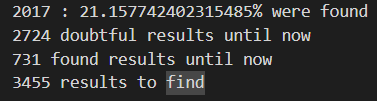
\includegraphics[width=7cm]{stats0.png}
    \caption{Statistiques de 2017 avant le téléchargement des PDFs}
\end{figure}

Pour finir, je devais faire une présentation de quelques slides afin de présenter mes résultats à l'équipe Gaia.
Un léger refactoring du code (division en plus de fonctions) et surtout sa documentation étaient également nécessaires. 
\\
Les résultats obtenus pour ce projet sont donc présentés sur les slides suivantes :

\begin{figure}[H]
    \centering
    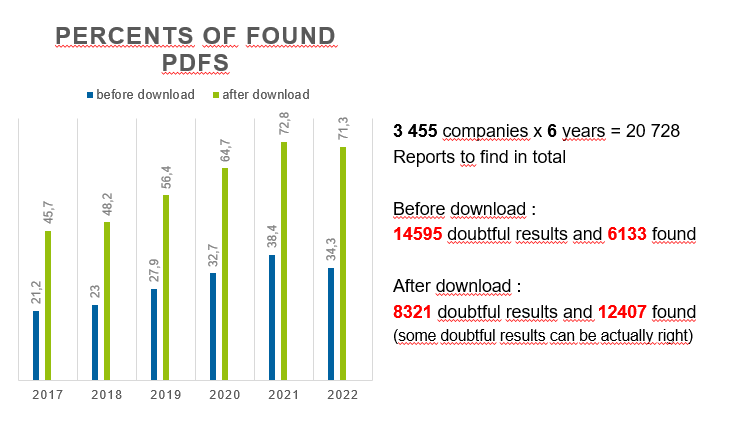
\includegraphics[width=\textwidth]{gaia_results.png}
    \caption{Résultats du projet GAIA (nombre de PDFS trouvés et douteux)}
\end{figure}

\begin{figure}[H]
    \centering
    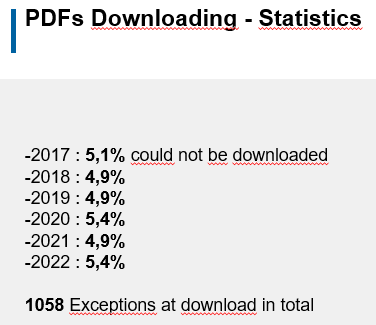
\includegraphics[width=8cm]{pdfs_not_downloaded.png}
    \caption{Statistiques sur les PDFs n'ayant pu être téléchargés}
\end{figure}

Ces résultats étaient donc plutôt bons et ont satisfait l'équipe Gaia.
 
\subsubsection{Projet ESCB Exchange}

\subsubsection{Projet CSDB}

\subsubsection{Projet NFIG}

\subsubsection{Projet de recherche NLP}

\subsection{Planning général suivi}